%!TEX root = ../presa.tex
\documentclass[12pt,pdf,hyperref={unicode}, dvipsnames]{beamer}
\usepackage[english,russian]{babel}
% \usepackage[T2A,T1]{fontenc}
\usepackage[utf8]{inputenc}
\usepackage{tikz}
\usepackage[unicode]{hyperref}
\usepackage{pgfplots,standalone}
% \usepackage{lmodern}
\pgfplotsset{compat=newest} 
\usetikzlibrary{%
    decorations.pathreplacing,%
    decorations.pathmorphing,%
    patterns,%
    angles,%
    quotes,%
    calc, %
    3d, %
    backgrounds, %
    positioning%
}

% Стиль презентации
\usetheme{Warsaw}

% \setbeamercolor{frametitle right}{fg=white,bg=Brown!85}
% \setbeamercolor{frametitle}{fg=white,bg=Brown!85}
\setbeamercolor{frametitle right}{fg=white,bg=black!95}
\setbeamercolor{frametitle}{fg=white,bg=black!95}

\setbeamertemplate{frametitle}[default][colsep=-4bp,rounded=false,shadow=false]
% \setbeamertemplate{frametitle}
% {
%     \nointerlineskip
%     \begin{beamercolorbox}[sep=0.3cm,ht=1.8em,wd=\paperwidth]{frametitle}
%         \vbox{}\vskip-2ex%
%         \strut\insertframetitle\strut
%         \vskip-0.8ex%
%     \end{beamercolorbox}
% }
\setbeamercolor{section in head/foot}{fg=white, bg=black}
\setbeamertemplate{frametitle}{%
    \nointerlineskip%
    \begin{beamercolorbox}[wd=\paperwidth,ht=2.5ex,dp=1.6ex]{frametitle}
        \hspace*{1ex}\insertframetitle%
    \end{beamercolorbox}%
}
\setbeamertemplate{headline}{}
\setbeamertemplate{footline}{}
\let\Tiny=\tiny % решает проблему со шрифтами в TexLive
% \setbeamertemplate
% 	{footline}{
% 		\color{black!40!white}
% 		\quad\hfill
% 		\insertframenumber/\inserttotalframenumber
% 		\hfill\vspace{1em}\quad
% 	} 

\setbeamertemplate{navigation symbols}{}

\beamersetrightmargin{0.5cm} 
\beamersetleftmargin{0.5cm}

\setbeamertemplate{enumerate item}{
	\usebeamercolor[bg]{item projected}
    \tikz[baseline = -4pt]{\draw[fill=black!95] (0,0) circle (3pt);}%
	% \raisebox{1pt}{\colorbox{bg}{\color{fg}\footnotesize\bf\insertenumlabel}}%
}
\setbeamertemplate{enumerate subitem}{ 
    \usebeamercolor[bg]{item projected}
    \tikz[baseline = -4pt]{\draw[fill=black!95] (0,0) circle (2.5pt);}%
    % \raisebox{1pt}{\colorbox{bg}{\color{fg}\footnotesize\bf\insertenumlabel.\insertsubenumlabel}}%
}
\setbeamercolor{item projected}{bg=black,fg=white}

% \setbeamertemplate{itemize item}{%
% 	\usebeamercolor[bg]{item projected}%
% 	\raisebox{1pt}{{\color{bg}\footnotesize$\bf\square$}}%
% }
% \setbeamercolor{item projected}{bg=black,fg=white}
\setbeamercolor{title}{bg=black,fg=white}

\newcommand\frametitless[1]{\subsection{#1}\frametitle{#1}}

\usepackage{booktabs, setspace}
\usepackage{esdiff,esint}
\newcommand{\tabitem}{~~\llap{\textbullet}~~}
\setbeamertemplate{caption}{\raggedright\insertcaption\par}
\title[]{Исследование нелинейных свойств высокотемпературных сверхпроводников с помощью ближнепольной СВЧ-микроскопии}
\institute{Радиофизический факультет ННГУ, 430 группа}
\date{Нижний Новгород, 2018}

\usepackage[font=footnotesize,justification=centering]{caption}
\captionsetup[figure]{labelformat=empty}%
% \setbeamertemplate{caption}[default]
\usefonttheme{professionalfonts}
\defbeamertemplate*{background canvas}{mydefault}
    {%
      \ifbeamercolorempty[bg]{background canvas}{}{\color{bg}\vrule width\paperwidth height\paperheight}% copied beamer default here
    }

    \defbeamertemplate*{background canvas}{bg}
    {%
      \color{black}\vrule width\paperwidth height\paperheight% added bg color
    }

    \BeforeBeginEnvironment{frame}{%
      \setbeamertemplate{background canvas}[mydefault]%
    }

    \makeatletter 
    \define@key{beamerframe}{bg}[true]{%
      \setbeamertemplate{background canvas}[bg]%
    }
    \makeatother

\newcommand{\sq}[1]{\tikz{\draw[draw=#1,fill=#1] (0,0) rectangle (0.7em,0.7em);}}
\usepackage{xcolor}
\definecolor{ochre}{HTML}{e2431e} % #e2431e 0
\definecolor{lightorange}{HTML}{e7711b} % #e7711b 1
\definecolor{lightyellow}{HTML}{f1ca3a} % #f1ca3a 2
\definecolor{lightgreen}{HTML}{6f9654} % #6f9654 3
\definecolor{osci}{HTML}{82FF27}%#82FF27
\definecolor{sky}{HTML}{1c91c0} % #1c91c0 4
\definecolor{violet}{HTML}{43459d} % #43459d 5

\begin{document}  
% \end{document}
%%%%%%%%%%%%%%%%%%%%%%%%%%%%%%%%%%%%%%%%%%%%%%%%%%%%%%%%%%%%%
\begin{frame}[plain]
	\centering
	\vspace{1.2cm}
	\begin{beamercolorbox}[sep=8pt,center]{title}
		\bf\usebeamerfont{title}\inserttitle
	\end{beamercolorbox}
	\vspace{0.5cm}
	\normalsize \textbf{Работу выполнили:}\\
	\large
	\underline{Сарафанов Ф.Г.}, %
	{Платонова М.В.}, %
	{Новиков А.Г.}
	% Рогов М.А. #wasted
	% Геликонова В.Г. % #wasted
	\\ 
	\vspace{0.5cm}
	\normalsize{\textbf{Научный руководитель:}\\}
	\large{Пестов Е.Е.}
	% \large{Яковлев А.И.}
	% \large{Антипов О.Л.}
	% \large{Щапин Д.С.}
	% \large{Мареев Е.А.}
	\vfill
	\small{Нижний Новгород -- 2018}
\end{frame}
%%%%%%%%%%%%%%%%%%%%%%%%%%%%%%%%%%%%%%%%%%%%%%%%%%%%%%%%%%%%%
% \begin{frame}[t]s
% 	\frametitle{Содержание}
% 	% \fontsize{6pt}{7.2}\selectfont
% 	\setbeamerfont{subsection in toc}{size=\tiny}
% 	\setbeamerfont{section in toc}{size=\tiny}
% 	\tableofcontents
% \end{frame}
%%%%%%%%%%%%%%%%%%%%%%%%%%%%%%%%%%%%%%%%%%%%%%%%%%%%%%%%%%%%%

\section{Введение}
\subsection{Цели работы}
\begin{frame}[t]
	\frametitle{Цели работы}
	% \textbf{Цели}\\
	\vfill
	\begin{spacing}{1}
		\begin{enumerate}
			\item Ознакомиться с моделью нейрона, обладающей свойствами генерировать  подпороговые колебания и импульсы возбуждения
			\item Феноменологически получить модельные уравнения и качественно исследовать их динамику
			\item Рассмотреть электронную схему, соответствующую модельным уравнениям
			\item Осуществить компьютерный и физический эксперименты, сравнить результаты
			% феноменологическая модель
		\end{enumerate}
	\end{spacing}
	\vfill
\end{frame}

\subsection{Сверхпроводимость}
\begin{frame}[t]%[bg]
	\frametitle{Основные свойства сверхпроводимости}
	\vspace{-1.5em}
	% \vspace{-0.5em}
	\begin{columns}
		\begin{column}{0.49\textwidth}%\centering
			\begin{figure}[h]
				% \hspace{-2em}
				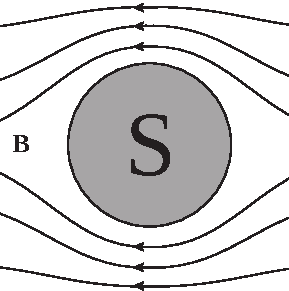
\includegraphics[width=0.5\linewidth]{img/messner}
				% \vspace{-0.5em}
				\caption{Эффект Мейснера}
			\end{figure}
			\vspace{-2em}
			\begin{figure}[h]
				% \hspace{-2em}
				% 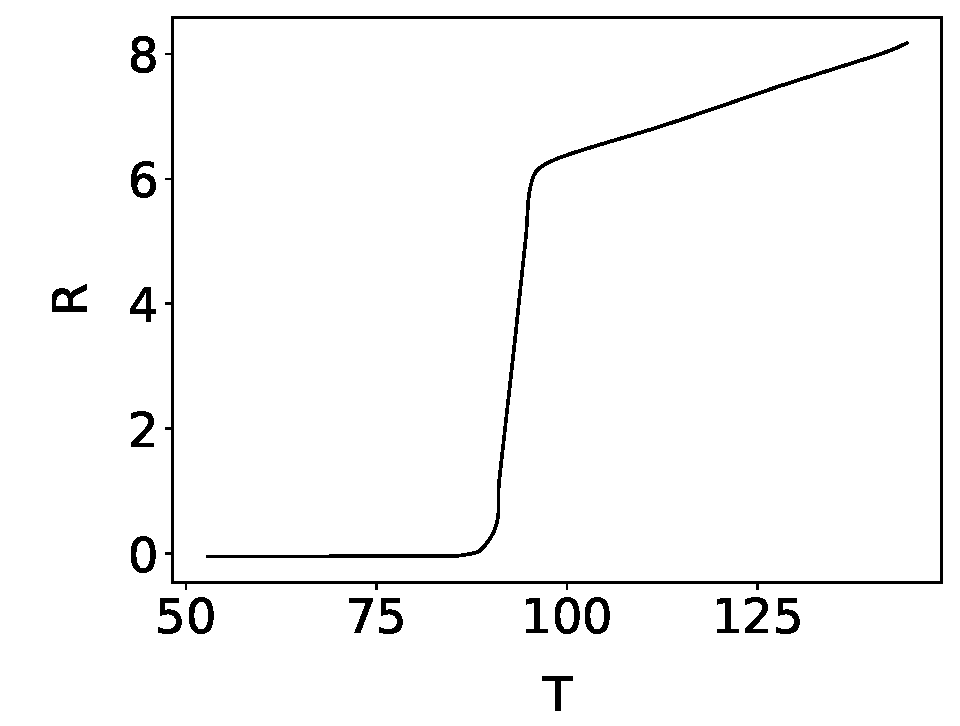
\includegraphics[width=0.8\linewidth]{pic/rt}
				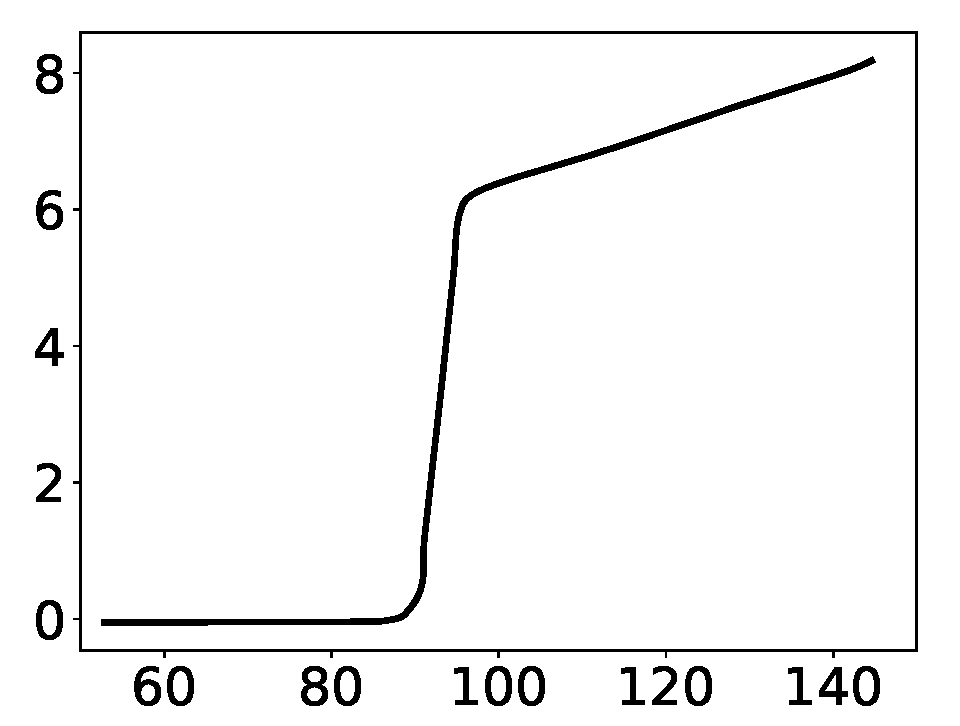
\includegraphics[width=0.8\linewidth]{pic/rt2}
				\vspace{-0.5em}
				\caption{Падение сопротивления до 0}
			\end{figure}
		\end{column}
		\begin{column}{0.49\textwidth}%\centering
			\begin{figure}[h]
				% \hspace{-2em}
				\vspace{-1em}
				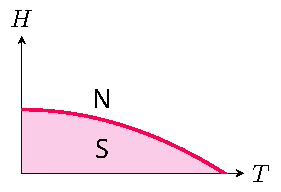
\includegraphics[width=0.8\linewidth]{pic/ns1}
				\vspace{-0.5em}
				\caption{Сверхпроводники 1-го рода}
			\end{figure}
			\vspace{-2em}
			\begin{figure}[h]
				% \hspace{-2em}
				% 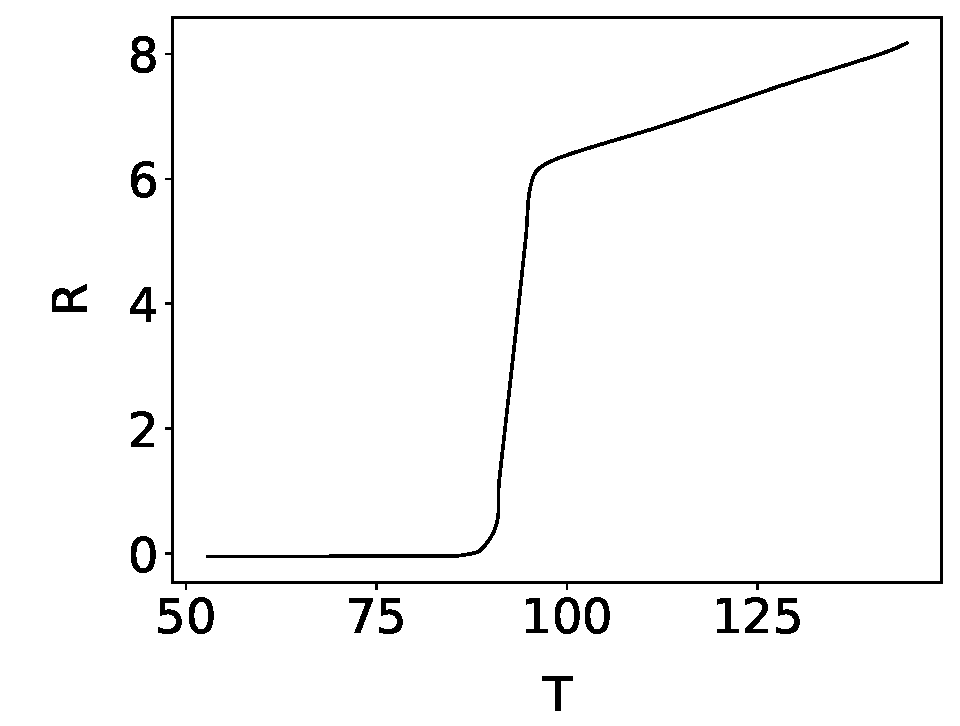
\includegraphics[width=0.8\linewidth]{pic/rt}
				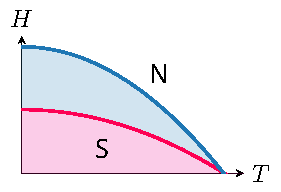
\includegraphics[width=0.8\linewidth]{pic/ns2}
				\vspace{-0.5em}
				\caption{Сверхпроводники 2-го рода}
			\end{figure}
		\end{column}
	\end{columns}		
\end{frame}

\subsection{Механизмы нелинейности сверхпроводников}
\begin{frame}[c]%[bg]
	\frametitle{Механизмы нелинейности сверхпроводников}
	% \vspace{-1em}
	% \vspace{-0.5em}
	\begin{enumerate}
		\item Нелинейность Гинзбурга-Ландау
		\item Тепловая нелинейность $n_s=n_s(T)$
		% Зависимость концентрации сверхпроводящих 
		% электронов от температуры
		\item Вихревая нелинейность
		\item Нелинейность Джосефсона
	\end{enumerate}
\begin{center}
	$\Downarrow$
\end{center}
% В приближении слабого сигнала выполняется феноменологическая формула нелинейности:
\begin{equation*}
	\vec{j}_s\sim\vec{A}\left(1-\frac{A^2}{A_c^2}\right)
\end{equation*}

	% \begin{columns}
	% 	\begin{column}{0.49\textwidth}%\centering
	% 		\begin{figure}[h]
	% 			% \hspace{-2em}
	% 			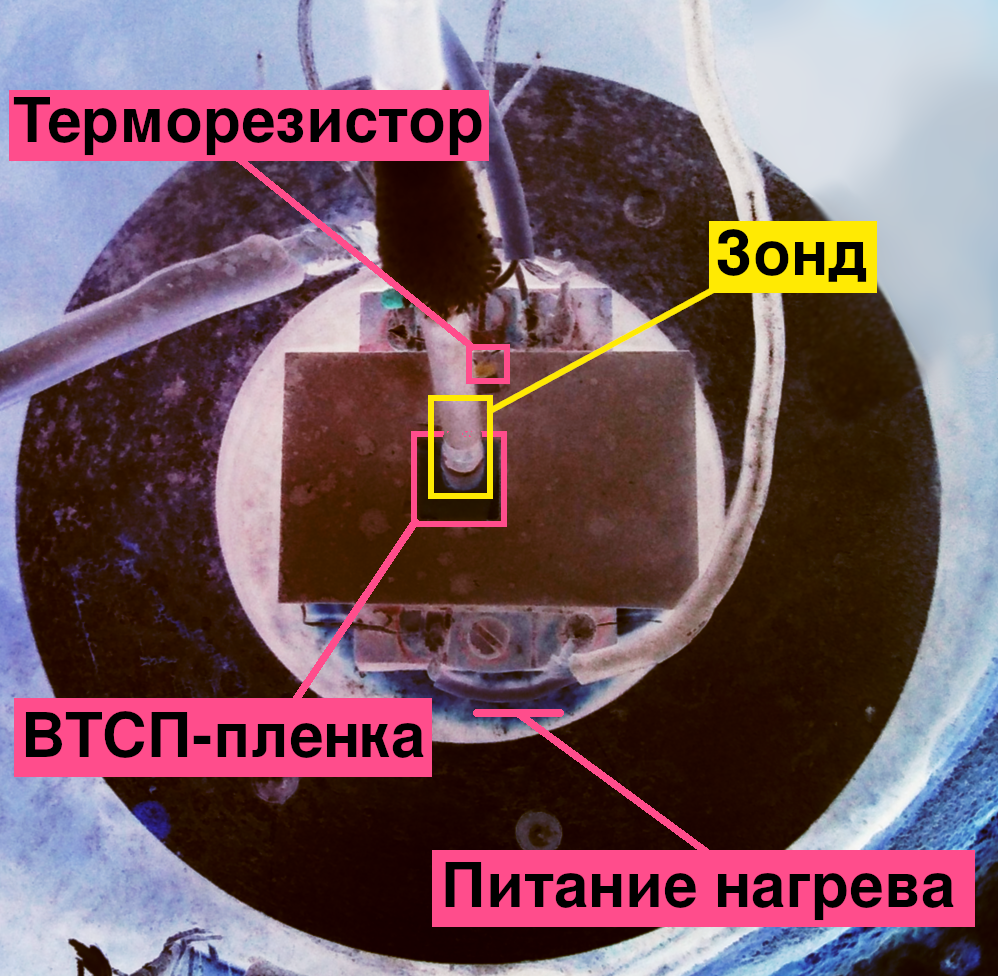
\includegraphics[width=0.86\linewidth]{img/above.png}
	% 			\caption{СВЧ-зонд над образцом с регулируемой температурой}
	% 			% \vspace{1em}
	% 		\end{figure}
	% 	\end{column}
	% 	\begin{column}{0.49\textwidth}%\centering
	% 		\begin{figure}[h]
	% 			% \hspace{-2em}
	% 			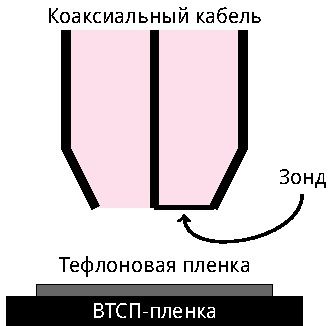
\includegraphics[width=0.86\linewidth]{pic/exp}
	% 			\caption{Конструкция ближнепольного СВЧ-зонда}
	% 		\end{figure}
	% 	\end{column}
	% \end{columns}		
\end{frame}

\subsection{Диаграмма температурных зависимостей}
\begin{frame}[c]%[bg]
	\frametitle{Диаграмма температурных зависимостей}
	% \vspace{-1em}
	% \vspace{-0.5em}
	\begin{figure}[H]
		\centering
		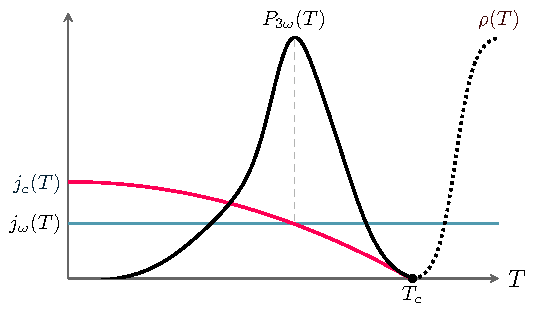
\includegraphics[scale=1.2]{pic/img_3a}
		% \caption{Caption here}
		\label{fig:chem}
	\end{figure}	
\end{frame}

\subsection{Блок-схема экспериментальной установки}
\begin{frame}[c]%[bg]
	\frametitle{Блок-схема экспериментальной установки}
	% \vspace{-1em}
	\vspace{-0.5em}
	\begin{figure}[H]
		\centering
		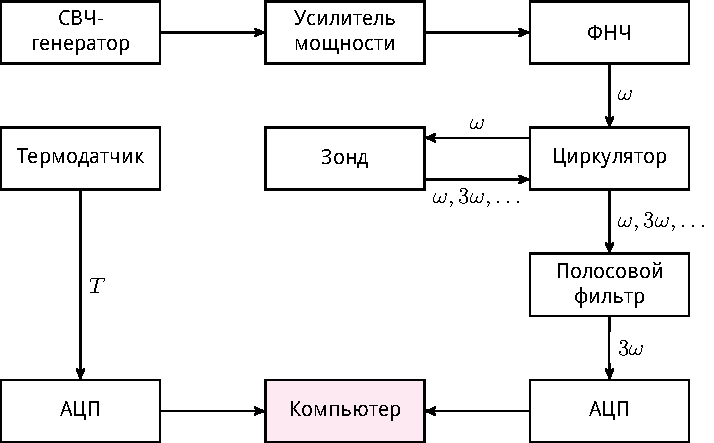
\includegraphics[]{pic/chem}
		% \caption{Caption here}
		\label{fig:chem}
	\end{figure}	
\end{frame}

\subsection{СВЧ-зонд}
\begin{frame}[c]%[bg]
	\frametitle{СВЧ-зонд}
	% \vspace{-1em}
	% \vspace{-0.5em}
	\begin{columns}
		\begin{column}{0.49\textwidth}%\centering
			\begin{figure}[h]
				% \hspace{-2em}
				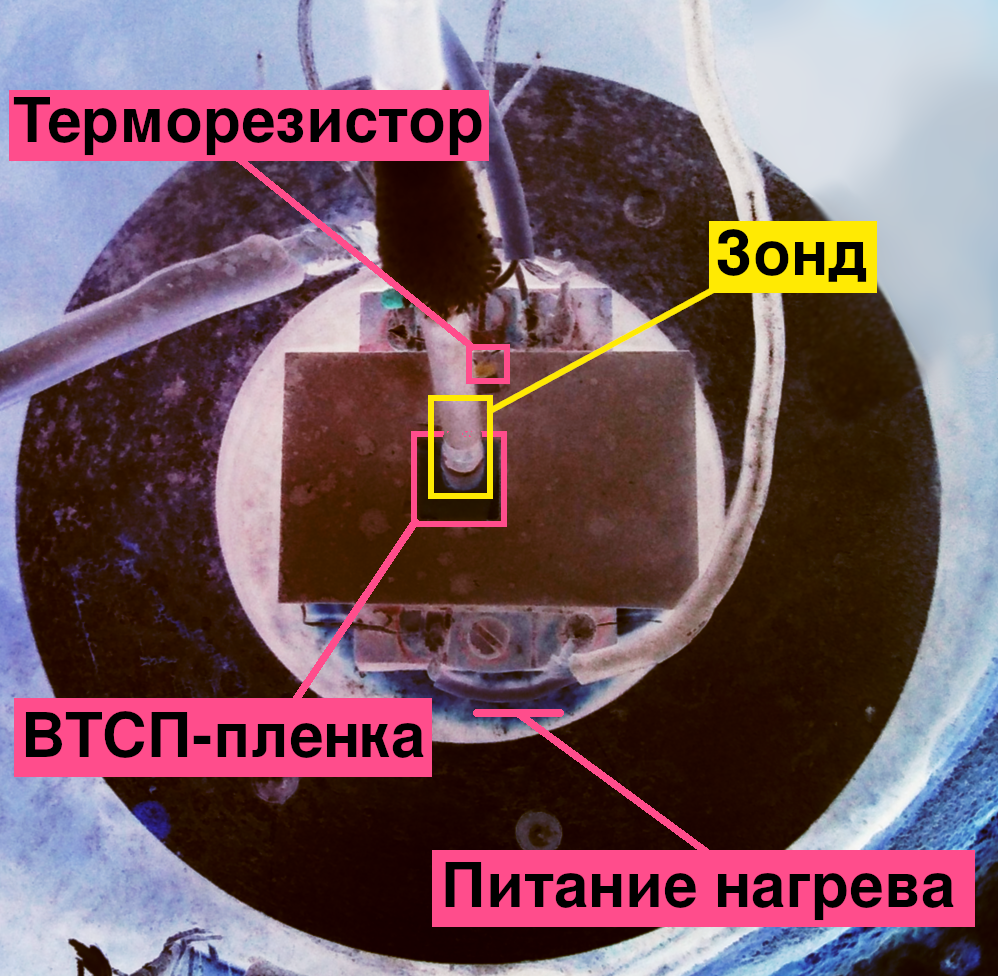
\includegraphics[width=0.86\linewidth]{img/above.png}
				\caption{СВЧ-зонд над образцом с регулируемой температурой}
				% \vspace{1em}
			\end{figure}
		\end{column}
		\begin{column}{0.49\textwidth}%\centering
			\begin{figure}[h]
				% \hspace{-2em}
				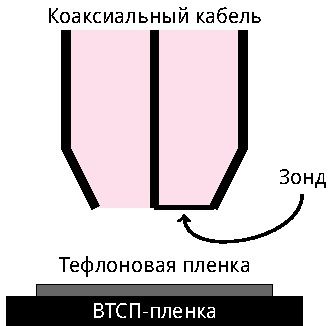
\includegraphics[width=0.86\linewidth]{pic/exp}
				\caption{Конструкция ближнепольного СВЧ-зонда}
			\end{figure}
		\end{column}
	\end{columns}		
\end{frame}


\subsection{Нелинейный отклик ВТСП-пленки}
\begin{frame}%[bg]
	\frametitle{Нелинейный отклик сверхпроводящей пленки}
	\begin{figure}[h]
		% \hspace{2em}
		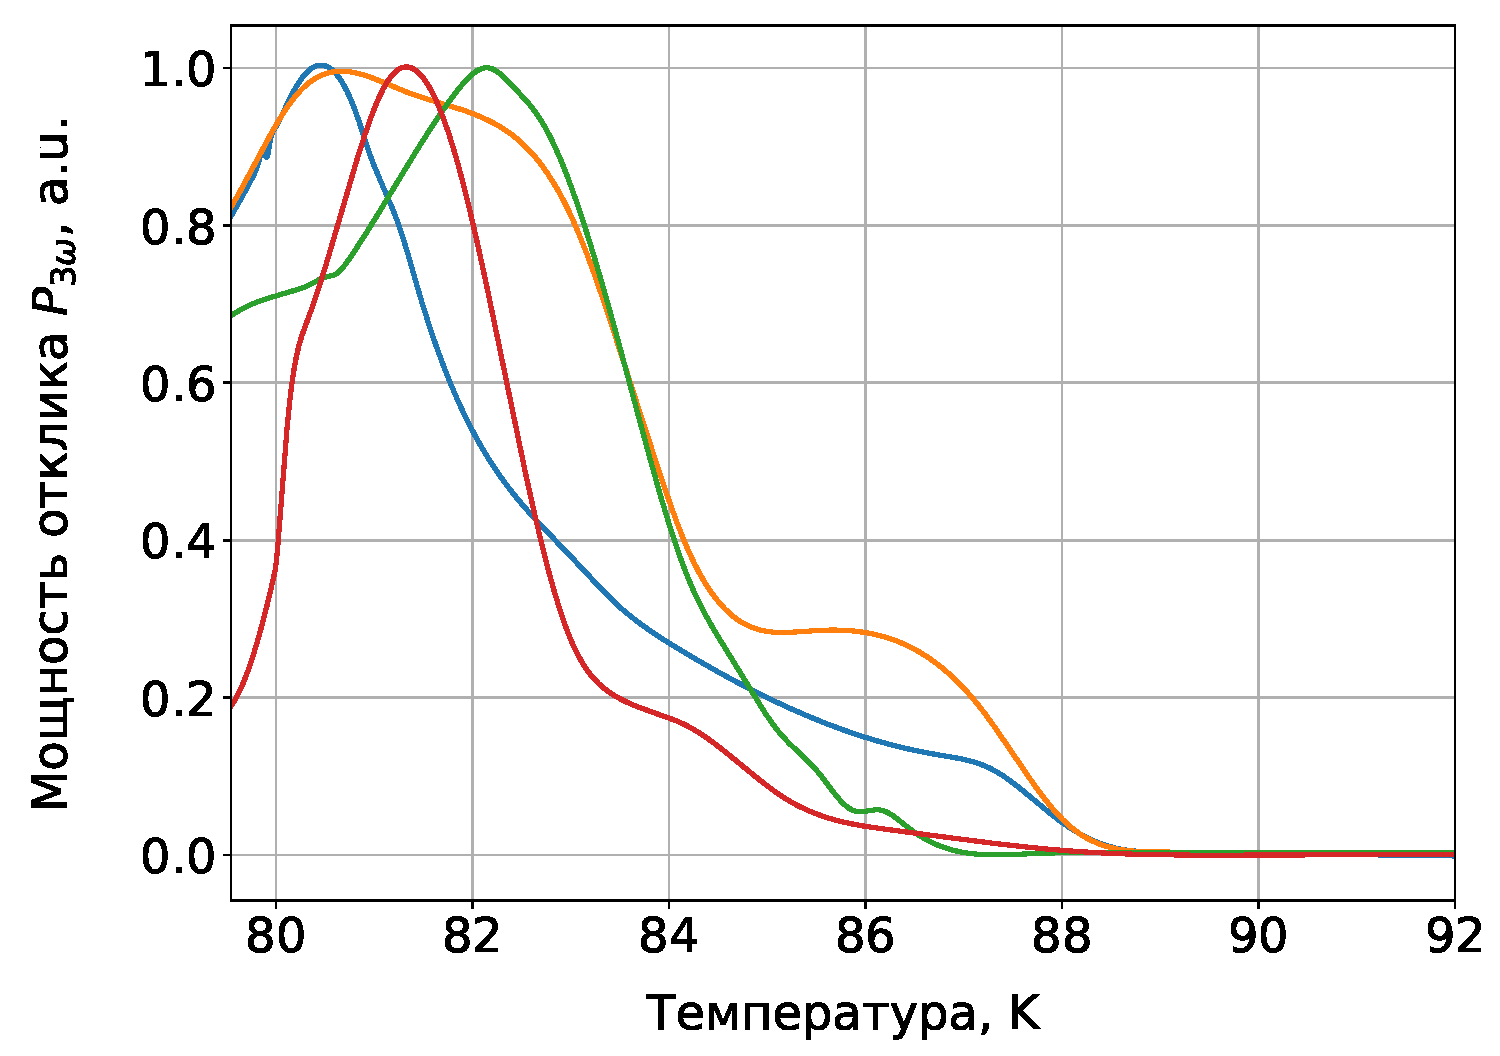
\includegraphics[width=0.9\textwidth]{pic/figg}
	\end{figure} 
\begin{tikzpicture}[remember picture,overlay]
\node at (9,6) {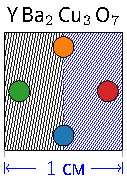
\includegraphics[scale=1]{pic/plenka}};
\end{tikzpicture}
\end{frame}

% %%%%%%%%%%%%%%%%%%%%%%%%%%%%%%%%%%%%%%%%%%%%%%%%%%%%%%%%%%%%%
\section{Заключение}
\subsection{Выводы}
\begin{frame}
	\frametitle{Выводы}
	\begin{enumerate}
		\item Изучены основные свойства сверхпроводников
		\item Методом ближнепольной СВЧ-микроскопии снята нелинейная зависимость мощности отраженного от ВТСП-пленки сигнала $P_{3\omega}(T)$, с помощью которой:
		\begin{enumerate}
		\item Определена средняя критическая температура и её пространственный разброс: $$\langle T_c\rangle_{S}=88.5\text{ K},\qquad T_c\in 87..89 \text{ K}$$
		\item Сделан вывод о наличии разных фаз сверхпроводимости в исследуемой ВТСП-пленке
		\item Качественно показана неоднородность $\vec{j}_\text{кр}$ в ВТСП-пленке
		\end{enumerate}
	\end{enumerate}
\end{frame}
% %%%%%%%%%%%%%%%%%%%%%%%%%%%%%%%%%%%%%%%%%%%%%%%%%%%%%%%%%%
\subsection{Спасибо за внимание}
\begin{frame}[plain]
	\vspace{4cm}
	\begin{center}
		\Huge
		Спасибо за внимание!
	\end{center}
	\vspace{2.5cm}
	\begin{center}
		\color{black!60!white}
		Презентация подготовлена в издательской \\
		системе LaTeX с использованием пакетов \\
		PGF/TikZ и Beamer
	\end{center}
\end{frame}
\end{document}